\section{Introduction}
\label{sec:intro}

Daylighting, the use of natural light for illumination, is clearly
beneficial in human-occupied
spaces~\cite{hhm15,Leslie03}.
Yet, daylighting design is dominated by passive window positioning
and configuration~\cite{Leslie03} rather than active control mechanisms,
except in a few cases~\cite{kt16}.

To explore the possibilities of actively controlled daylighting systems,
a catoptric (mirror-based) surface has recently been installed in
the south facing glass fa\c cade of a campus building
(see Figure~\ref{fig:steinberg})~\cite{acadia18}.
The catoptric surface is comprised of 650 mirrors, each with 2 independent
degrees of freedom (pan and tilt), providing a full hemisphere
range of motion.

With 256 possible positions per degree of freedom (180\degree{} range
and 0.7\degree{} resolution), 2 degrees of freedom per mirror, and 650 mirrors, 
there are over 300,000 possible stable configurations of the catoptric surface.
Add to this the desire to control mirror movement profiles (i.e.,
acceleration), and the number of configurations grows considerably.

In this paper, we describe our approach to controlling the catoptric surface
as a device on the Internet of Things (IoT).
The control is decomposed hierarchically, with low-level controllers
(locally)
handling individual mirror motions and high-level control (remotely)
managing the
desired position (and movement profiles) of the set of mirrors.

\begin{figure}[ht]
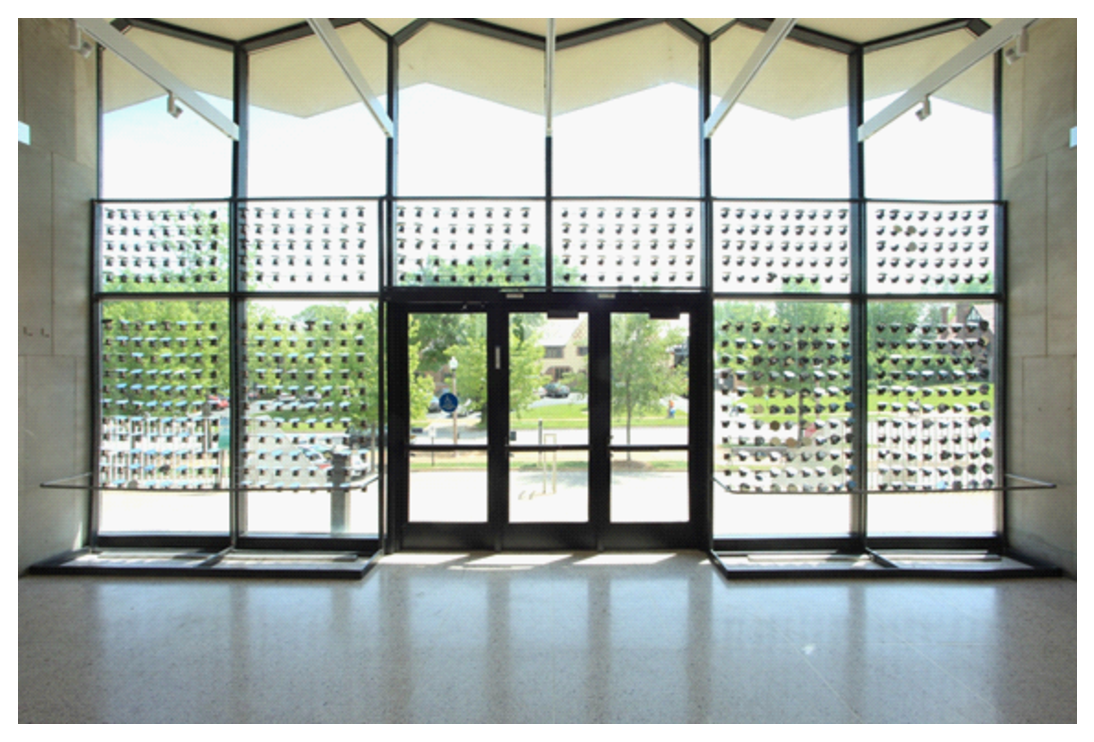
\includegraphics[width=0.88\columnwidth]{steinberg}
\caption{Array of mirror units inside of the south-facing glass fa\c cade, Steinberg Hall, Washington Univ.~in St.~Louis~\protect\cite{acadia18}.}
\label{fig:steinberg}
\end{figure}


